\documentclass[a4paper]{article}
\usepackage{graphicx}
\usepackage[comma]{natbib}
\usepackage{apalike} 
\bibliographystyle{named}
\setcitestyle{aysep={,}}
\usepackage{amsmath, amsthm, amsfonts, amssymb, amscd, bm, breqn}
\usepackage{dsfont}
\usepackage{verbatim}
\usepackage{url}
\usepackage[hidelinks]{hyperref}
\usepackage[table,xcdraw]{xcolor}
\usepackage{float}
\usepackage{enumerate}
\usepackage{enumitem}
\usepackage[noabbrev,capitalize]{cleveref}
\usepackage[font=footnotesize,labelfont=bf,width=0.8\textwidth]{caption}
\usepackage{subcaption}


% !TeX spellcheck = en_GB

%\textwidth = 6.2 in≠
\textheight = 9 in
\topmargin = 0.0 in
	\addtolength{\oddsidemargin}{-.575in}
	\addtolength{\evensidemargin}{-.575in}
	\addtolength{\textwidth}{1.15in}
%\headheight = 0.0 in
%\headsep = 0.0 in
\parskip = 0.1in
% \parindent = 0.2cm

\newcommand{\N}{\mathbb{N}}
\newcommand{\R}{\mathbb{R}}
\newcommand{\Z}{\mathbb{Z}}
\newcommand{\Q}{\mathbb{Q}}
\newcommand{\bs}[1]{\boldsymbol{#1}}
\newcommand{\y}{\boldsymbol{y}}

% \newcommand\numberthis{\addtocounter{equation}{1}\tag{\theequation}}

\begin{document}

% \title{Ellipsoid Criterion}
\title{A Multivariate Extension to the Standard 4$\sigma$ Criterion for Comparison of Forensic Glass Evidence}
\author{Oliver Lountain}

\maketitle

\section*{Abstract}
\label{sec:abstract}
\addcontentsline{toc}{section}{\nameref{sec:abstract}}



\tableofcontents


\section{Introduction}

\subsection{Forensic Glass Evidence}

When a person breaks a glass object -- such as a window --  minuscule fragments of the broken glass are transferred to the person's clothing. This process of fragmentation of the broken glass back towards the object which broke it was observed by \citet{Nelson1967} and is now referred to as backscatter fragmentation. Any person within ``a few feet of the window" which is broken will likely have a number of minute fragments of glass transferred to their clothing. When a suspect is apprehended, these fragments can be found on their clothing and compared to the glass which was broken, potentially placing the suspect close to the object at the crime scene when it was broken. This analysis requires a careful treatment as one of course wishes to avoid wrongfully convicting an innocent person. As such, the development of measurement techniques with a high level of precision to discriminate between, say, two panes of glass manufactured at the same factory, on the same day, but installed as windows in two distinct buildings is of the utmost importance.

\subsection{LA-ICPMS Data}

Multiple methods have been used over time to measure glass evidence, including the colour, thickness and refractive index of the glass \citep{Curran2000}, though more recently, the elemental composition has been the preferred approach. Elemental composition offers a multivariate measurement of the data, and as such can allow for a greater level of discrimination between samples. In Australia, LA-ICPMS \citep{Houk1990,Curran1997,Aeschliman2003,Weis2011,Trejos2013,Dorn2015} is conducted in some forensic laboratories and so data collected in this way will be the focus of this paper, though the techniques discussed can be applied to any elemental composition measurements. The motivation behind our research stems from the question of whether the currently employed interval-based criterion can be improved upon to take full advantage of the multivariate elemental data.

\subsection{Data sets}

We consider two data sets: a homogeneous set of observations taken from two glass factories in the USA and a much more diverse set of observations originating from South Australian casework from 2017 to 2020.

\subsubsection*{USA Ribbon Data}

This first, homogeneous, data set was commissioned to serve as a database of chemical composition measurements by \citet{Park2019}. The data is comprised only of measurements of float glass manufactured by two companies in the United States of America. These companies will be referred to as Company A and Company B. A sample of 31 panes of float glass was taken from Company A, labelled $AA, AB, \dots, AAR$, and 17 manufactured by Company B labelled $BA, BB, \dots, BR$. The panes sampled from Company A were manufactured between the third and 24th of January, 2017, and those produced by Company B were sampled a little earlier from the fifth to the 16th of December, 2016 \citep{Park2020}. 

Glass is manufactured in long continuous sheets known as ribbons, which are then cut into panes. At both of these factories, a large number of samples were taken from each ribbon of glass in order to develop an understanding of the level of variability within a source. To achieve this, on almost all days within the sampling periods, for both manufacturers, two glass panes were collected -- one from each side of the ribbon. A sample of 24 fragments were then taken from each pane, and from 21 of these fragments, five replicate measurement were taken. For the other three, 20 replicate measurements were made, resulting in a total of 165 measurements per pane of glass.

In this study, the choice of elements to measure was made following \citet{Weis2011}, who recommended that only 18 elements are used. Three major elements: calcium, sodium and magnesium; three minor elements: aluminium, potassium and iron; and 12 trace elements: lithium, titanium, manganese, rubidium, strontium, zirconium, barium, lanthanum, cerium, neodymium, hafnium, and lead.

\subsubsection*{Australian Casework Data}

The second data set comprises glass collected during casework in South Australia which has been measured and analysed by FSSA. The measurements in this data set span from 2016 to 2020 at the time of writing, and as the data is from real police casework, there is some variability in the number of measurements obtained. The data also come in two distinct forms: control samples and recovered samples. Control samples are taken from a known source at the scene of the crime, and typically at least nine individual fragments are measured, and between one and three replicate measurements are made of each fragment, depending on what is possible given the size of the fragment. Recovered samples are typically those taken from suspects' clothing as well as other sources such as the interior of a car. These samples are much less numerous, with between one and three fragments measured, and again between one and three replicate measurements for each fragment. Given that these observations are far less numerous and do not have a known source, only control fragments are considered for the analysis throughout in order to maintain a certain level of consistency in the observations used.


\section{Match Criteria}

The standard practice by forensic practitioners for comparing glass samples with LA-ICPMS elemental analysis is via some interval-based match criteria \citep{Park2019}. Specifically, two international standards are used: \citet{ASTM12} and \citet{ASTM16}. In this setting, we consider glass from a known source at a crime scene, referred to as the control source, and a glass sample obtained from a suspect's clothing, known as a recovered source. To simplify the notation, we will denote the known and questioned samples by $\bs{y}_1$ and $\bs{y}_2$ respectively. For each sample, the concentrations of $p$ elements are measured, for $n_l$ fragments of a given sample of broken glass (where $l=1,2$). In some cases there will also be replicate measurements taken of each fragment. In order to avoid over-complicated notation, we assume that replicate measurements are contained in the index spanning the number of fragments. That is, we take $n_l$ to span the fragments and replicates for sample $l$. In full, the control and recovered measurements are denoted 
$$
\bs{y} = \left\{y_{ljk} \, | \, l = 1,2, j = 1,\dots,n_l, k = 1,\dots,p \right\}.
$$
From this, we have that each measurement is a vector of the form
\begin{equation*}
	\bs{y}_{lj} = (y_{lj1}, \dots, y_{ljp}).
\end{equation*}
The mean vector for each element in sample $l$ is then denoted
\begin{equation*}
    \bar{\bs{y}}_l = \frac{1}{n_l} \sum_{j=1}^{n_l} \bs{y}_{lj},
\end{equation*}
and similarly the vector of standard deviations is
\begin{equation*}
    \bs{\sigma}_l = \frac{1}{n_l-1} \sum_{j=1}^{n_l} (\bar{\y} - \bs{y}_{lj})^2.
\end{equation*}
That is,
\begin{equation*}
	\bar{\bs{y}}_l = (\bar{y}_{l1}, \dots, \bar{y}_{lp}),
\end{equation*}
and
\begin{equation*}
	\bs{\sigma}_l = (\sigma_{l1}, \dots, \sigma_{lp}),
\end{equation*}

\subsection{Standard 4$\sigma$ Interval Criterion}

%Trejos2013a in the first citation

Starting with the standard criterion \citep{Koons2002,ASTM12,ASTM16}, we consider two glass samples $\bs{y}_{1}$ and $\bs{y}_{2}$, where $\bs{y}_{1}$ is from a known source and $\bs{y}_{2}$ is the sample in question. The guidelines suggest that at least nine measurements be taken from the known source via three replicates of three fragments and that ``as many measurements as are practical" be taken of the sample in question \citep{ASTM16}. Comparison intervals are then constructed for each element individually. The $k$-th comparison interval is computed as the mean of the control sample plus or minus four times its standard deviation. However, a lower bound is placed on the standard deviation of 3\% of the mean. As such, the $k$-th comparison interval is defined as 
\begin{equation}
\label{eqn:interval}
\bar{y}_{1k} \pm 4 \times \max\left\{ \sigma_{lk}, 0.03 \times  \bar{y}_{1k}\right\}.
\end{equation}

In other words, no matter the number of measurements obtained for the known fragment, the variability in this data can never be less than 3\% of the control mean. The concentrations of each of the $p$ elements in the questioned sample are then compared to the intervals calculated in \autoref{eqn:interval}. If the concentrations lie within the interval for all elements, then $\bs{y}_{1}$ and $\bs{y}_{2}$ are said to be chemically indistinguishable. In the event that one or more concentration lies outside its respective interval for any of the measurements, the samples are said to be chemically distinguishable. Equivalently, the distinction between two samples is quantified with a score determined by rearranging \cref{eqn:interval}. That is, we take the absolute difference between the concentrations of a the $k$-th element for the two samples and scale by the standard deviation of $\bs{y}_{1}$. We denote this by $S_{ASTM,k}$. The overall comparison score between the samples, denoted $S_{ASTM}$, is then taken to be the maximum across the $p$ elements.
\begin{equation}
\label{eqn:score}
S_{ASTM,k} = \left| \frac{\bar{y}_{1k} - \bar{y}_{2k}}{\max\left\{ \sigma_{1k}, 0.03 \times  \bar{y}_{1k}\right\}} \right|.
\end{equation}
\begin{equation*}
    S_{ASTM} = \max_{1 \leq k \leq p} S_{ASTM,k}.
\end{equation*}
This score exceeding four is equivalent to the questioned sample lying outside of the comparison interval and so the samples are declared distinguishable in this case \citep{ASTM12,ASTM16}.

\subsection{Ellipsoid 4$\sigma$ Criterion}

The interval-based criteria are most intuitively thought of as $p$ individual univariate tests. However, geometrically, this is equivalent to constructing a hyper-rectangle around the observations whose dimension is the number of elements measured. This hyper-rectangle would be located at the centroid of the data, and the length in each dimension would be $8\sigma$. Then, a recovered sample is declared as matching if it lies within this hyper-rectangle, and non-matching if it lies outside. The construction of this hyper-rectangle assumes no relationship between any of the elements. Therefore, the most natural extension of the standard interval criterion to take into account correlations between the elements would be to consider a $p$-dimensional ellipsoid centred about the mean vector. We would then wish for this ellipsoid to be rotated such that its principal axes align with the directions of greatest variation, and that the surface is always four standard deviations from the centre. As far as the author is aware, there is no mention of this in the forensic science literature, though it can be constructed quite easily by employing the Mahalanobis distance. The Mahalanobis distance is an example of what is known as a statistical distance, and provides a well-defined notion of distance between observations. To define it, let $\bs{X}$ and $\bs{Y}$ be two random vectors from the same distribution with covariance matrix $\Sigma$. Then the Mahalanobis distance $d_M(\bs{X},\bs{Y})$ between $\bs{X}$ and $\bs{Y}$ is given by 
\begin{equation*}
    d_M(\bs{X},\bs{Y}) = \sqrt{(\bs{X}-\bs{Y})^T \Sigma^{-1} (\bs{X}-\bs{Y})}.
\end{equation*}
The Mahalanobis distance is a generalisation of Euclidean distance, scaled by the standard deviation in the direction between the two points. As a result, the numerical value of the Mahalanobis distance is precisely the number of standard deviations between the two points. It is worth noting also that in one dimension, the Mahalanobis distance simplifies precisely to the standard $4\sigma$ score as expressed in \cref{eqn:score}. Further, by considering a centroid $\bs{\mu}$ and an observation $\bf{x}$, both in $\R^p$, a $p$-dimensional ellipsoid centred at $\bs{\mu}$, whose distance from the edge to the centre is equal to $r$ standard deviations is given by the equation
\begin{equation*}
    \label{eqn:stdev_ellipsoid}
    \left(d_M(\bs{\mu},\mathbf{x})\right)^2 =  (\bs{\mu}-\mathbf{x})^T \Sigma^{-1} (\bs{\mu}-\mathbf{x}) = r^2.
\end{equation*}
This is referred to as the standard deviational ellipsoid and any point which lies within this hyper-ellipsoid is within $r$ standard deviations of the mean vector, $\bs{\mu}$. Thus, by classifying matches for comparisons where the Mahalanobis distance is less than four, and non-matches where it is greater than four, this provides a natural generalisation of the standard $4\sigma$ interval method. For control and recovered samples $\y_1$ and $\y_2$, the comparison score in this case is therefore given by
\begin{equation*}
    S_{\text{ellipsoid}} = d_M(\bs{y}_1,\bs{y}_2).
\end{equation*}

% To understand why this works, first consider that the general equation for an ellipsoid centred at $\bs{w} \in \R^p$ is
% \begin{equation*}
%     \left(\bs{w} - \bs{u}\right)^T A \left(\bs{w} - \bs{u}\right) = 1,
% \end{equation*}
% where $\bs{u},\bs{w} \in \R^p$ and $A$ is a $p \times p$ positive definite matrix. Here, $A$ defines the scale and rotation of the ellipsoid. Let $\lambda_1,\dots,\lambda_p$ be the eigenvalues of $A$. Then the semi-axes of the ellipsoid are given by $\lambda_1^{-2},\dots,\lambda_p^{-2}$. The eigenvectors of $A$ then define the principal axes of the ellipsoid, that is, its rotation in $\R^p$. Now, in the context of data, we note that the eigenvectors of $\Sigma$ define the principal components of the data, that is, the orthogonal vectors of greatest variance. The corresponding eigenvalues then provide the size of the deviation in each respective direction. Let $\bs{s}_1,\dots, \bs{s}_p$ be the eigenvectors  and $\varsigma_1^2,\dots ,\varsigma_p^2$ the eigenvalues of $\Sigma$. Here, $\varsigma_i^2$ is the variance in the $i$-th principal component. Then, since $\Sigma$ is symmetric and invertible, $\bs{s}_1,\dots, \bs{s}_p$ are the eigenvectors of $\Sigma^{-1}$ also, and $\varsigma_1^{-2},\dots ,\varsigma_p^{-2}$ are its eigenvalues. Thus, since $\Sigma^{-1}$ is also positive definite, we have that the equation 
% \begin{equation*}
%     (\bs{\mu}-\mathbf{x})^T \Sigma^{-1} (\bs{\mu}-\mathbf{x}) = 1
% \end{equation*}
% defines a $p$-dimensional ellipsoid centred at $\bs{\mu}$, with principal axes $\bs{s}_1,\dots, \bs{s}_p$, and semi-axes $\varsigma_1,\dots ,\varsigma_p$. Finally, we can rewrite \cref{eqn:stdev_ellipsoid} as
% \begin{equation*}
%     (\bs{\mu}-\mathbf{x})^T r^{-2} \Sigma^{-1} (\bs{\mu}-\mathbf{x}) = 1.
% \end{equation*}
% The matrix $r^{-2} \Sigma^{-1}$ has the same eigenvectors as $\Sigma$, and has eigenvalues $r^{-2}\varsigma_1^{-2},\dots ,r^{-2}\varsigma_p^{-2}$. Therefore, we have that \cref{eqn:stdev_ellipsoid} defines a $p$-dimensional ellipsoid centred at $\bs{\mu}$, with principal axes $\bs{s}_1,\dots, \bs{s}_p$, and semi-axes $r\varsigma_1,\dots , r\varsigma_p$. That is, each semi-axis has length $r$ standard deviations.

To help visualise the distinction between the standard and ellipsoid $4\sigma$ criteria consider \cref{fig:ellipse}. The data used in this figure has been simulated to clearly demonstrate the potential distinction. To keep the visualisation simple, only two variables have been used. Variables 1 and 2 have been simulated from a bivariate normal distribution, with covariance matrix given by
\begin{equation*}
    \begin{bmatrix}
        1 & 0.5 \\ 0.5 & 1
    \end{bmatrix}.
\end{equation*}
The black points show the simulated data, the straight black lines show the boundaries for the standard criterion in each variable, and the black ellipse is that for a Mahalanobis distance of four. The red cross shows a new observation which would be declared as matching by the standard criterion, but rejected by the ellipsoid method, while the opposite is true for the blue cross.



\begin{figure}[h]
	\centering
	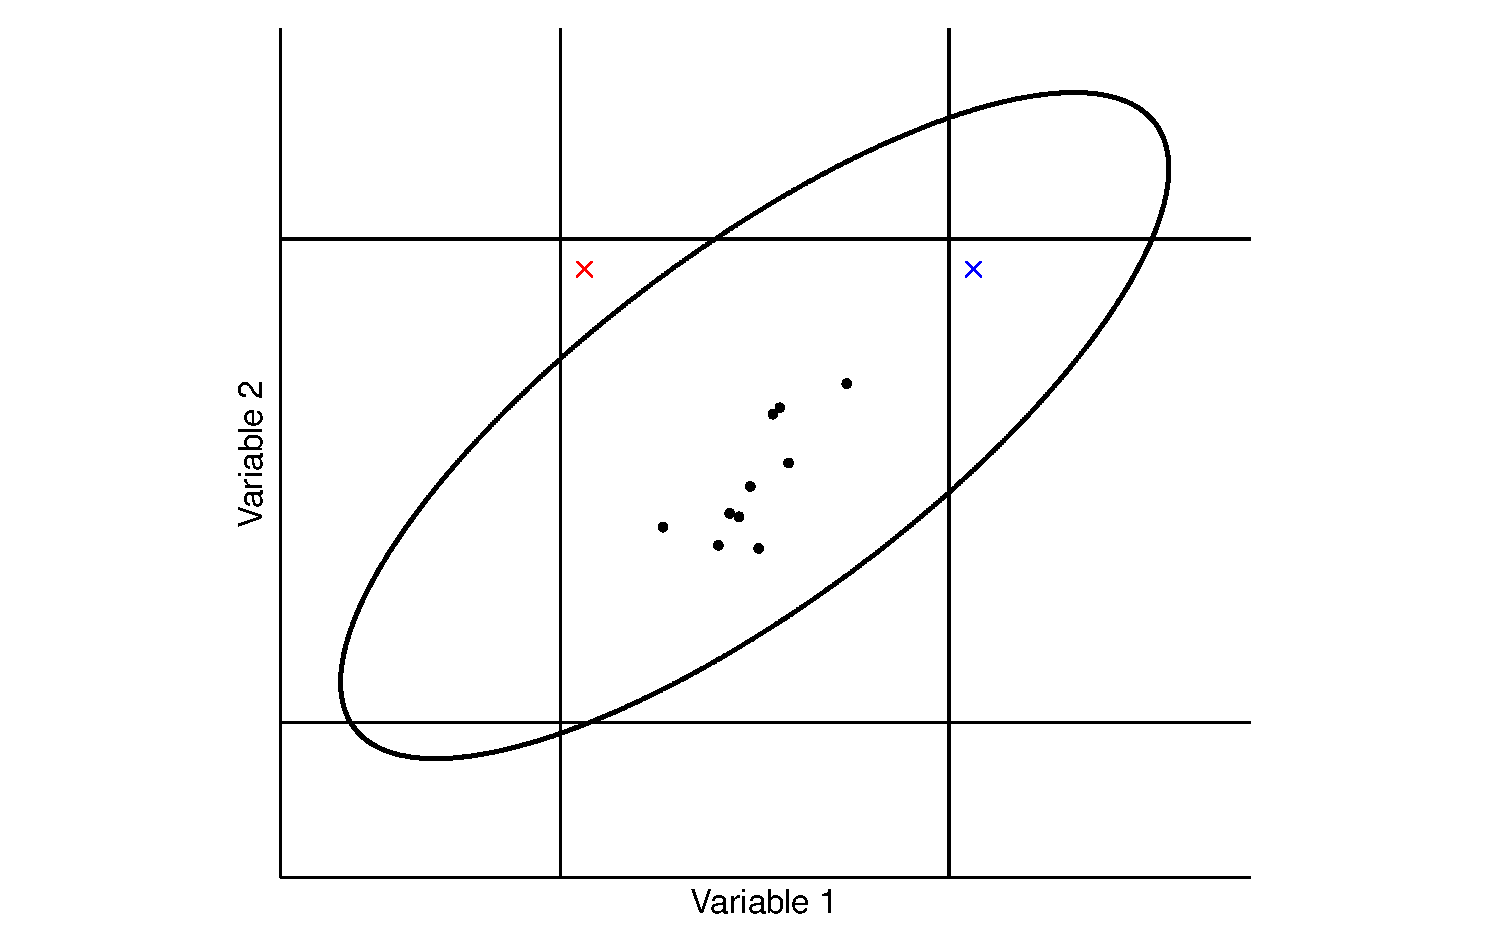
\includegraphics[width=0.8\linewidth]{figures/ellipse.eps}
	\caption{Comparison of standard and ellipsoid $4\sigma$ match criteria in two variables. Variables 1 and 2 have been simulated from a bivariate normal distribution, each with variance 1, and the covariance is 0.5. The black points show the simulated data, the straight black lines show the boundaries for the standard criterion in each variable, and the black ellipse is that for a Mahalanobis distance of four. The red cross shows a new observation which would be declared as matching by the standard criterion, but rejected by the ellipsoid method, while the opposite is true for the blue cross.}
	\label{fig:ellipse}
\end{figure}


\section{Results}


\subsection{USA Ribbon Data}

We begin by applying the two methods to the USA ribbon data. We note in \cref{tab:std_metrics_usa} that the standard $4\sigma$ criterion was only approximately 60\% accurate, and that its low value of kappa suggests little difference between it and a uniform random classifier. It received a perfect score for sensitivity, meaning that it never incorrectly classified matching pairs as non-matching, but received quite a low score for specificity, meaning a large number of false positive predictions. The ellipsoid $4\sigma$ criterion appears to have significantly improved upon the standard method, achieving a raw accuracy of 0.950. It also scored above 0.9 for both sensitivity and specificity, with specificity in particular scoring above 0.95, meaning that false positives were minimised.

\begin{table}[h]
	\centering
    \begin{tabular}{lrrrr}
        \hline
		method       & accuracy  & kappa      & sensitivity & specificity \\ \hline
        Standard $4\sigma$ & 0.616 & 0.109 & 1.000 & 0.600\\
		Ellipsoid $4\sigma$  & 0.950 & 0.575 & 0.917 & 0.951\\ \hline
	\end{tabular}
	\caption{Performance metrics for standard and ellipsoid $4\sigma$ criterion applied to USA ribbon data. The standard criterion is only approximately 60\% accurate while the ellipsoid criterion is 95\% accurate. The standard criterion scored 0.109 for Cohen's Kappa, suggesting only a slight improvement over a uniform classifier, while the ellipsoid criterion received a score of 0.575 The standard criterion received a perfect score for sensitivity, meaning that it never incorrectly classified matching pairs as non-matching, but received quite a low score for specificity, meaning a large number of false positive predictions. The ellipsoid criterion has high scores for both sensitivity and specificity, with both above 90\%.}
	\label{tab:std_metrics_usa}
\end{table}

To provide another interpretation of sensitivity and specificity, we see that the standard $4\sigma$ criterion predicted perfectly on same source pairs, but only 60\% of the time on different source pairs. The ellipsoid criterion, by contrast, predicted correctly 91.7\% of the time on same source pairs, and 95\% of the time on different source pairs. In other words, the ellipsoid criterion sacrifices approximately 8\% accuracy on same source pairs, in order to increase different source accuracy by 35 percentage points.

\subsection{Australian Casework Data}

Moving on to the Australian casework data, \cref{tab:std_metrics_aus} displays the performance metrics of these two criteria on this data set. We see that in terms of raw accuracy, both methods perform quite well, with the ellipsoid criterion performing slightly better with a near-perfect score of 0.992, an increase of 0.031 over the standard criterion. In Cohen's kappa coefficient, the difference is more pronounced, with a significant increase of 0.34 from the standard to ellipsoid criterion, suggesting that accounting for correlations has a significant impact on classification as compared to a random classifier. Looking at sensitivity and specificity, we note that the standard criterion achieves a perfect score for sensitivity, suggesting that it predicted no false negatives, that is, no pairs of fragments were classified as non-matching, when they were in fact matching. The standard criterion traded this high sensitivity for a slightly lower specificity, suggesting that it made a small number of false positive predictions. The ellipsoid criterion, achieved a balance with  close to perfect scores for both sensitivity and specificity.

\begin{table}[h]
	\centering
    \begin{tabular}{lrrrr}
        \hline
		method       & accuracy  & kappa      & sensitivity & specificity \\ \hline
        Standard $4\sigma$ & 0.961 & 0.497 & 1.000 &  0.960\\
		Ellipsoid $4\sigma$  & 0.992 & 0.837 & 0.990 & 0.992\\ \hline
	\end{tabular}
	\caption{Performance metrics for standard and ellipsoid $4\sigma$ criterion applied to Australian data. In terms of raw accuracy, both methods perform quite well, with the ellipsoid criterion performing slightly better with a near-perfect score of 0.992, an increase of 0.031 over the standard criterion. In Cohen's kappa coefficient, the difference is more pronounced, with a significant increase of 0.34 from the standard to ellipsoid criterion, suggesting that accounting for correlations has a significant impact on classification as compared to a random classifier. We note also that the standard criterion achieves a perfect score for sensitivity, suggesting that it predicted no false negatives.}
	\label{tab:std_metrics_aus}
\end{table}

The score of 1.000 for sensitivity means that the standard $4\sigma$ criterion performed perfectly on same source pairs, and the specificity shows that it correctly predicted 96\% of the time on different source pairs. By contrast, the ellipsoid $4\sigma$ criterion made correct predictions 99\% of the time on same source pairs, and 99.2\% of the time on different source pairs.


\section{Discussion}

Overall, we note that both the standard and ellipsoid criteria perform quite well on the diverse Australian casework data set, with the ellipsoid method offering substantial improvement on different source classifications. The standard criterion performed quite poorly on the homogeneous USA ribbon data, being able to classify same sources pairs as matching, but struggling to correctly classify different source pairs. The ellipsoid method, taking into account the correlation structure between the variables, closed this gap and offered substantial improvement on different source classification, while maintaining good performance on same source comparisons.

\addcontentsline{toc}{section}{References}
\bibliography{../../../MPhil/Research/Bibliography/full_bibliography}


\end{document}